\documentclass[compactaffiliation]{Interspeech}

% Interspeech paper kit: https://www.overleaf.com/latex/templates/interspeech-paper-kit/kzcdqdmkqvbr
\interspeechcameraready

\usepackage{booktabs}
\usepackage{array}
\usepackage{url}
\usepackage{tikz}
\usetikzlibrary{arrows.meta,positioning}

\title{Assignment 1: Unimodal Baselines for Hateful Memes}
\author[affiliation={1}]{Pavel}{Adamov}
\affiliation{}{Johannes Kepler University Linz}{Austria}
\email{Student ID: K12336734}
\keywords{hateful memes, unimodal baselines, frozen encoders, linear classifier}

\begin{document}

\maketitle
\hypersetup{pdfauthor={Pavel Adamov}}

\begin{abstract}
We train four unimodal baselines for classifying memes as hateful or non-hateful: two image
encoders (CLIP ViT-B/16, DINOv2-base) and two text encoders (all-mpnet-base-v2, RoBERTa-base). Each
encoder is frozen and followed by a single linear layer. With the same search budget and three
seeds per model, CLIP reaches a validation AUROC of 0.657, MPNet 0.650, RoBERTa 0.621 and DINOv2
0.571. CLIP is clearly better than DINOv2, while the best image and text models perform about the same.
\end{abstract}



\section{Encoders}
We use two image and two text encoders (Table~\ref{tab:encoders}), all loaded from Hugging Face and
kept frozen. The two image encoders were trained in different ways. CLIP \cite{radford2021clip}
was trained on images paired with captions, so its features describe what an image shows and it
can partly read text inside images. DINOv2 \cite{oquab2024dinov2} was trained on images only and
mainly describes visual appearance. The two text encoders also differ: all-mpnet-base-v2
\cite{reimers2019sbert, song2020mpnet} was trained to produce sentence embeddings, while RoBERTa
\cite{liu2019roberta} is a general language model that was not trained for this purpose.

\begin{table}[b]
\caption{Encoders, all from Hugging Face. The short commit identifies the exact weights.}
\label{tab:encoders}
\centering\scriptsize
\setlength{\tabcolsep}{2.5pt}
\begin{tabular}{@{}l >{\raggedright\arraybackslash}p{4.15cm} c >{\raggedright\arraybackslash}p{1.45cm}@{}}
\toprule
Name & Model, checkpoint (commit) & Dim & Pooling \\
\midrule
Image A & CLIP ViT-B/16, \texttt{openai/clip-vit-base-patch16} (57c2164) & 512 & projected pooled output \\
Image B & DINOv2 ViT-B/14, \texttt{facebook/dinov2-base} (f9e44c8) & 768 & CLS token after final norm \\
Text A & MPNet, \texttt{sentence-transformers/ all-mpnet-base-v2} (e8c3b32) & 768 & masked mean \\
Text B & RoBERTa, \texttt{FacebookAI/roberta-base} (e2da8e2) & 768 & masked mean \\
\bottomrule
\end{tabular}
\end{table}

\begin{table*}[t]
\caption{Four-model comparison. Validation AUROC is the mean $\pm$ sample standard deviation over seeds 0, 1, 2;
the 95\% bootstrap interval is for the seed 0 model. The test set has no labels, so test AUROC is not available (n/a).}
\label{tab:results}
\centering\footnotesize
\begin{tabular}{llccc}
\toprule
Baseline & Encoder checkpoint & Test AUROC & Val AUROC & 95\% CI (val) \\
\midrule
Image A & \texttt{openai/clip-vit-base-patch16} & n/a & 0.657 $\pm$ 0.004 & [0.605, 0.700] \\
Image B & \texttt{facebook/dinov2-base} & n/a & 0.571 $\pm$ 0.002 & [0.521, 0.618] \\
Text A & \texttt{sentence-transformers/all-mpnet-base-v2} & n/a & 0.650 $\pm$ 0.002 & [0.600, 0.698] \\
Text B & \texttt{FacebookAI/roberta-base} & n/a & 0.621 $\pm$ 0.002 & [0.573, 0.672] \\
\bottomrule
\end{tabular}
\end{table*}

\begin{table*}[t]
\caption{Validation memes on which the image model (Img, CLIP) and the text model (Txt, MPNet)
disagree at a threshold of 0.5. Label 1 is hateful. Scores are from the seed 0 models.}
\label{tab:errors}
\centering\footnotesize
\begin{tabular}{rccc>{\raggedright\arraybackslash}p{12.4cm}}
\toprule
ID & Label & Img & Txt & Explanation \\
\midrule
82509 & 0 & 0.18 & 0.76 & The text refers to a stereotype about Muslim terrorists, but the image shows a fashion show. The meme is labelled non-hateful. The text model only sees the text and gives a false positive. \\
90843 & 0 & 0.18 & 0.76 & A pun on the word ``Hispanic'' over a photo of fast food, labelled non-hateful. The text model reacts to the ethnic word without the harmless image (false positive). \\
73914 & 1 & 0.58 & 0.08 & The text alone is harmless. The meme is hateful because it compares a Black child to a gorilla, which is a racist insult that can only be seen in the image. The text model misses it. \\
90243 & 1 & 0.68 & 0.19 & ``6 million kills'' next to a photo of Hitler refers to the Holocaust. Without the image the text reads like a gaming joke; the image model recognises Hitler. \\
13647 & 1 & 0.70 & 0.29 & ``Get back in the kitchen'' is sexist even without the image. The text model still gives a low score, probably because the sentence contains no insulting words. CLIP may read the large text in the image. \\
\bottomrule
\end{tabular}
\end{table*}

\section{Data and preprocessing}
We use the provided splits of the course dataset \cite{kiela2020hateful}: \texttt{train.jsonl} for
training (8{,}500 memes: 3{,}050 hateful, 5{,}450 non-hateful), \texttt{dev.jsonl} for validation
(500 memes: 250 hateful, 250 non-hateful) and \texttt{test.jsonl} as the test set (1{,}000 memes,
no labels provided).

The image models receive only the image pixels, prepared with each model's own preprocessing (CLIP:
resize the shorter side to 224, centre crop to 224, CLIP normalisation; DINOv2: resize the shorter
side to 256, centre crop to 224, ImageNet normalisation). No separate text is given to the image
models, but the text written on the meme is still visible in the image. The text models receive
only the meme text, processed with their own tokenizer (maximum length 128 tokens, longer texts
truncated, padding to the longest text in the batch). The text embedding is the average of the last
hidden layer over all non-padding tokens. Embeddings are computed once and saved (Figure~\ref{fig:pipeline}).

\begin{figure}[!h]
\centering
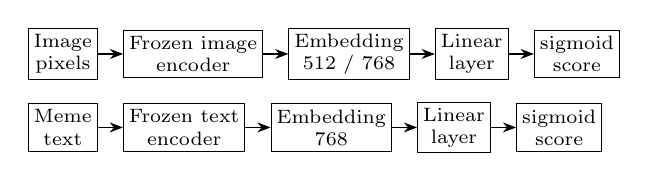
\begin{tikzpicture}[node distance=3.2mm, >=Stealth,
  box/.style={draw, rectangle, minimum height=6mm, align=center, font=\scriptsize, inner sep=2pt}]
  \node[box] (img) {Image\\pixels};
  \node[box, right=of img] (ie) {Frozen image\\encoder};
  \node[box, right=of ie] (ie2) {Embedding\\512 / 768};
  \node[box, right=of ie2] (lin1) {Linear\\layer};
  \node[box, right=of lin1] (s1) {sigmoid\\score};
  \node[box, below=3mm of img] (txt) {Meme\\text};
  \node[box, right=of txt] (te) {Frozen text\\encoder};
  \node[box, right=of te] (te2) {Embedding\\768};
  \node[box, right=of te2] (lin2) {Linear\\layer};
  \node[box, right=of lin2] (s2) {sigmoid\\score};
  \foreach \a/\b in {img/ie, ie/ie2, ie2/lin1, lin1/s1, txt/te, te/te2, te2/lin2, lin2/s2}
    \draw[->] (\a) -- (\b);
\end{tikzpicture}
\caption{Pipeline. The four models are trained and evaluated separately; modalities are never combined.}
\label{fig:pipeline}
\end{figure}

\section{Training}
Each classifier is a single linear layer with one output logit; only the input size changes between
models. We use hateful $=1$ and non-hateful $=0$, train with binary cross-entropy on the logit
(\texttt{BCEWithLogitsLoss}), and use $\sigma(\text{logit})$ as the hateful score. Features are
scaled with the training set mean and standard deviation. We use Adam \cite{kingma2015adam} with
batch size 256 for up to 100 epochs and keep the epoch with the highest validation AUROC.
Regularisation is L2 weight decay. All four models use the same 12 settings: learning rate in
$\{10^{-4},10^{-3},10^{-2}\}$ and weight decay in $\{0,10^{-4},10^{-2},10^{-1}\}$. The best setting is
chosen by validation AUROC with seed 0 and then trained with seeds 0, 1 and 2. All four models chose
learning rate $10^{-2}$ and weight decay $10^{-1}$; the kept epochs for seeds 0/1/2 were 75/49/25
(Image A), 90/18/93 (Image B), 39/43/98 (Text A) and 94/68/40 (Text B).

\section{Results}
AUROC is computed from the hateful scores, not from thresholded predictions, with the same code and
the same memes for all four models (Table~\ref{tab:results}). The test set has no labels, so test AUROC
cannot be computed and we report validation AUROC instead. These values are slightly optimistic,
because the validation set was also used to choose the settings and the epoch. The 95\% interval
comes from 2{,}000 bootstrap resamples of the 500 validation memes \cite{efron1993bootstrap}.



\section{Analysis}
\textbf{Within each modality.} CLIP is clearly better than DINOv2 (0.657 versus 0.571); the paired
bootstrap interval for the difference, [0.021, 0.143], does not include zero. A likely reason is
that CLIP features describe content such as people, symbols and partly the written text, while
DINOv2 features describe appearance, which says little about whether a meme is hateful. MPNet
scores higher than RoBERTa (0.650 versus 0.621), possibly because it was trained to produce sentence
embeddings, but the interval for this difference, [$-$0.028, 0.080], includes zero, so we cannot say
for certain that MPNet is better.

\textbf{Image versus text.} The best image model (CLIP) and the best text model (MPNet) perform about
the same; the interval for their difference is [$-$0.053, 0.060]. The small standard deviations over
seeds only show that training is stable; the uncertainty from having only 500 validation memes is
much larger. The image results do not measure purely visual understanding: the meme text is part of
the image and CLIP can partly read it, and the model may also learn which kinds of photos often
appear in hateful memes. In addition, the dataset contains memes where the same text or image is
used in both a hateful and a harmless meme \cite{kiela2020hateful}, so the label often depends on
the combination, which neither model sees. At a threshold of 0.5 the two models disagree on 145 of
the 500 validation memes.

\textbf{Error analysis.} We inspected five validation memes on which CLIP and MPNet disagree, taking
the three hateful and the two non-hateful memes with the largest difference between the two scores
(Table~\ref{tab:errors}). A fixed threshold of 0.5 is used for this analysis only; AUROC does not
use a threshold. Scores come from the seed 0 models.



\section{Reproducibility and acknowledgements}
The code is available at
\begin{center}\vspace{-2mm}\small\url{https://github.com/pavelavis/hateful-memes-unimodal-baselines}\vspace{-2mm}\end{center}
It contains a README, dependencies, the configuration with all settings and seeds, the commands for
feature extraction, training and evaluation, the trained classifiers and the encoder commits. Model
weights: OpenAI CLIP, Meta DINOv2, sentence-transformers MPNet and FacebookAI RoBERTa, all from
Hugging Face. Libraries: PyTorch, Hugging Face Transformers and scikit-learn. All scripts were
written for this project.

\bibliographystyle{IEEEtran}
\bibliography{refs}

\end{document}
